%************************************************
\chapter{The Business Tier}
\label{ch:business-tier}
%************************************************

\section{Introduction}

In the previous chapter, we have looked at what happens in the client tier (on the user device) and in the presentation tier (on the server side). We have seen the \ac{MVC} pattern in details and seen how it can be applied to generate dynamic HTML pages on the server side. We have seen that this pattern does not involves three components, but four: in addition to the \emph{model}, the \emph{view} and the \emph{controller}, there is also a \emph{service}. The role of the service is gather data and to apply business logic to generate the model, which is finally rendered by the view.

\marginpar{While it is possible to implement business services with POJOs, we introduce the notion of managed component. It allows the container to apply various policies (pooling, security, transactions, etc.).}

This chapter focuses on this type of component and describes how it can be implemented with \ac{Java EE} technologies. As always, there are different solutions and every solution has benefits and drawbacks. In the second part of the book, we will see how business services can be implemented with \ac{POJO}s managed by an application framework like Spring. In this part of the book, we present the approach recommended by the \ac{Java EE} specification, namely the use of \ac{EJB}s.

\section{Enterprise Java Beans}

The use of \ac{EJB}s has been a heated topic in the developer community and many discussions can be found on that subject in online forums. The accuracy of the arguments in these debates vary a lot and need to be taken with a grain of salt. 

\marginpar{When you implement an application with Java EE, you do not have to use EJBs. When you build an application with the Spring framework, you do use some of the Java EE technologies.}

For instance, one often hear statements like ``I don't want to use \ac{EJB}s, therefore I don't want to use \ac{Java EE}, therefore I will use something more lightweight like the Spring Framework''. \emph{This statement is incorrect!} The \ac{EJB} specification is one of the many specifications that are part of the \ac{Java EE} umbrella specification. It sits at the same level as the Servlet API or the \ac{JSP} specification. Deciding to use \ac{Java EE} to build an application does not mean that every single sub-specification \emph{has to} be used. Depending on the functional and non-functional requirements, the developer has to select the components that make sense in a given context. Coming back to the statement, as we will see in the second part of the book, the Spring Framework is built on top of technologies that are in the \ac{Java EE} scope. Spring applications can be packaged in .war files and deployed in application servers. \emph{Hence, when building a web application with the Spring framework, one does use some of the \ac{Java EE} APIs}.

\subsection{Opinions on EJBs: perceptions vs facts}

\marginpar{Be careful when reading articles about a platform that has evolved over 20 years. What was true in the early days might be very different today.}

When seeking for opinions on \ac{EJB}s in online forums and blog posts, one also need to be careful about the date when the comments were made. Both the \emph{specification} and the \emph{implementations} of \ac{EJB}s have changed dramatically since the beginning and we are talking about a technology that has matured over 15 years:

\begin{itemize}
\item  The evolution of the \emph{specification} has a big positive impact on the developer experience. Developing \ac{EJB}s with the first versions of the specification was a tedious projects. Several Java and XML files had to be created for every single business component. With the current specification, creating an \ac{EJB} can be done by adding a single annotation in a single Java file. The version 3.0 of the specification, which was part of Java EE 5, was a major shift which happened in 2006.
\item The evolution of the implementations has a positive impact on systemic qualities and particularly on performance. As we will see, \ac{EJB}s handle a lot tasks behind the scenes and it is not surprising that calling an \ac{EJB} is more expensive than calling a \ac{POJO}. Twenty years ago, the performance overhead was much more perceptible than it is today. 
\end{itemize}

Online archives can give the perception that \ac{EJB}s are still a pain to use and slow, but often people just repeat what they have heard and read. Only experiments with up-to-date environments can give the real picture. \ac{EJB} may not be the best choice for a given project, but the decision to use or not to use them should be based on facts rather than impressions. This comment applies to any architectural decision.

\subsection{The original vision}

The authors of the \ac{EJB} specification wanted to define a standard way to create and operate business services. Business-focused developers would create independent components, such as a customer management service, an inventory management service or an order management service. When creating these components, the developers would focus purely on the business logic and not deal with any user interface concern. The set of business components could then be used in two ways:

\begin{itemize}
\item they could be combined to create a complete \emph{enterprise application package}. Concretely, every business service would be packaged in an \emph{\ac{EJB} module} (a \texttt{.jar} file). Several of these modules would be added to an \emph{enterprise archive} (an \texttt{.ear} file). A \texttt{.war} file, packaging presentation-tier components would also be added to the enterprise archive. In this scenario, the development team would provide a big \texttt{.ear} file to the IT operations team, which would deploy it into an application server (or rather into a cluster of application servers).
\item they could also be deployed individually into the application server. A fundamental aspect of the original vision was that \ac{EJB}s would be \emph{distributed} components, exposing a remote interface. Hence, it should be possible for an application component in any tier to locate and invoke these business services. For instance, a rich client application should be able to make remote calls to an \ac{EJB} without going through servlets. Also, one \ac{EJB} running on a machine should be able to make remote calls to another \ac{EJB} running elsewhere.
\end{itemize}

\marginpar{In general, developers package all components together and deliver an application package. Since Java EE 6, it is not mandatory to use the .ear format: EJBs can be packaged in a .war file.}

The two scenarios are shown in Figures \ref{fig:deploymentEar} and \ref{fig:deploymentEjb}. In the first case, a complete enterprise package has been created and it is deployed across the cluster as a unit. Note that every \ac{EJB} may still expose a remote interface and be accessed from any application server node and from client machines. But in the normal flow, HTTP requests are processed by components in the \texttt{.war} package, which generates calls to \ac{EJB}s in the \texttt{.jar} files. In the second case, the \texttt{.war} and individual \texttt{.jar} files are deployed individually. Benefits of this approach is that services can be updated and redeployed with greater autonomy, and that flexible scaling strategies are possible. However, they come at the cost of increased complexity. The bottom line is that you make the choice to deploy an \ac{EJB} module as an independent unit, there must be a clear reason to do it.
\begin{figure}[]
	\centering
    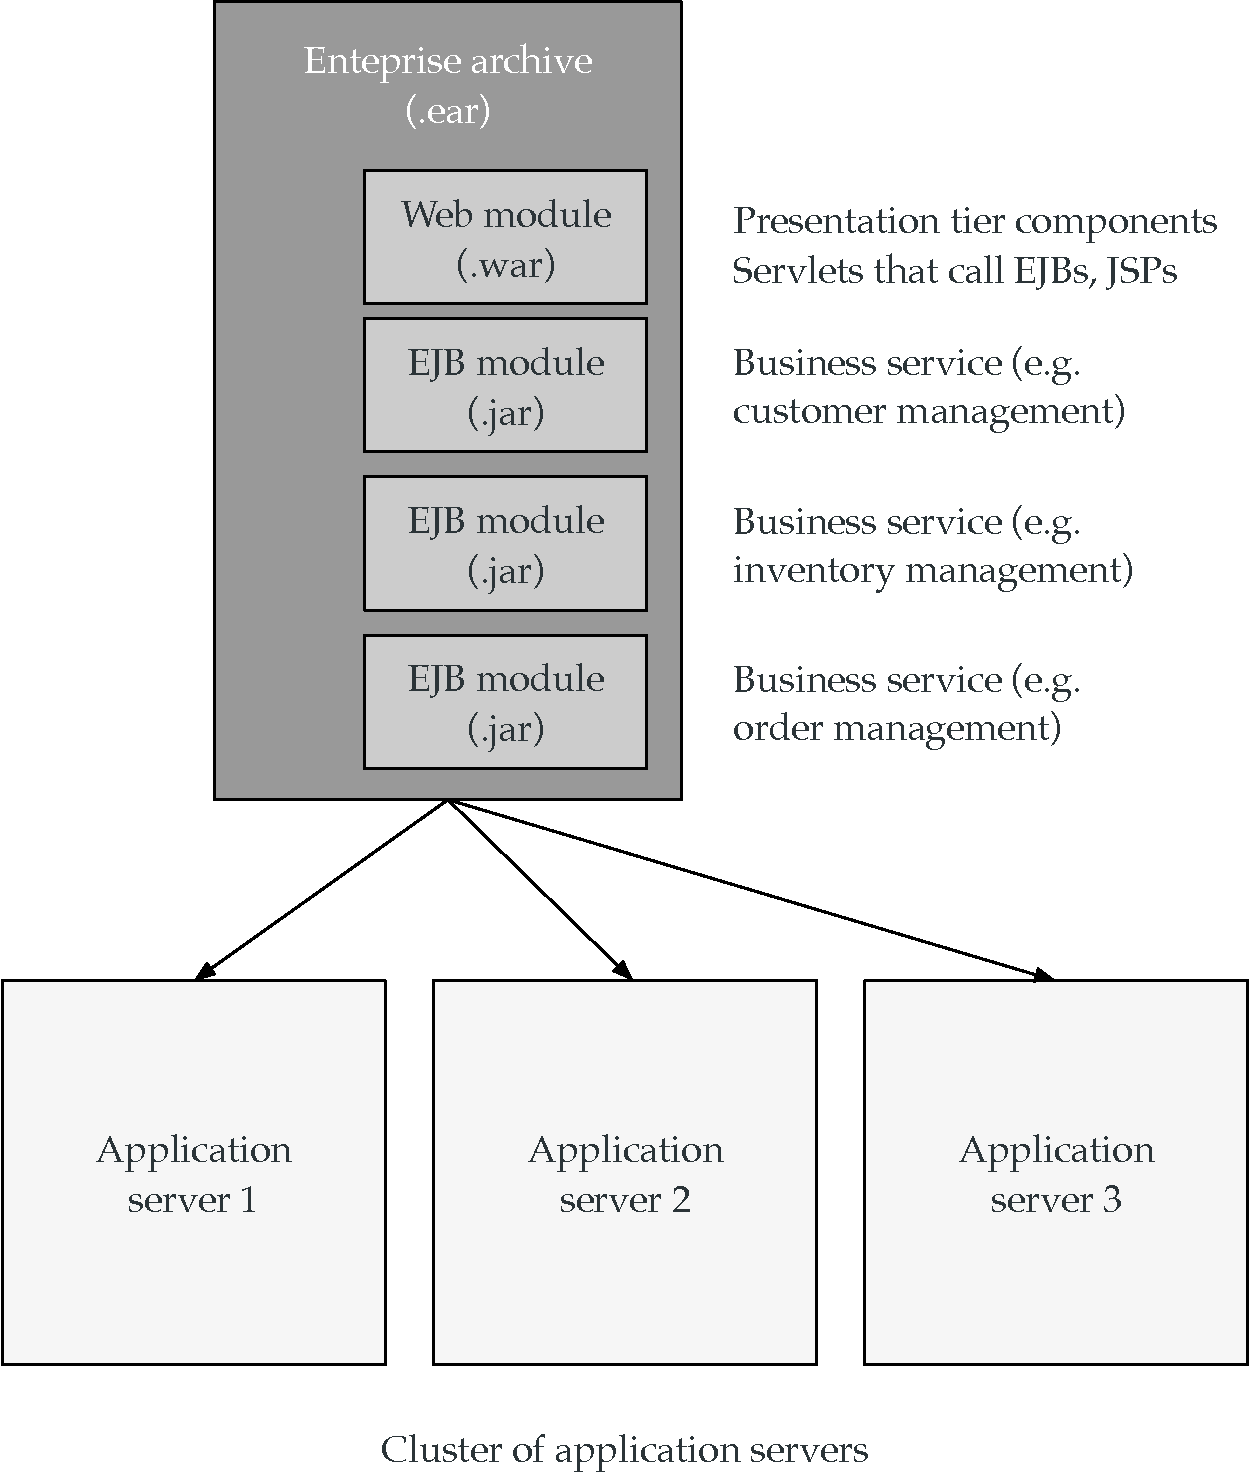
\includegraphics[width=0.8\linewidth]{Figures/deployment-ear.pdf}
	\caption{Deployment of a complete enterprise application in a cluster}
  \label{fig:deploymentEar}
\end{figure}

\begin{figure}[]
	\centering
    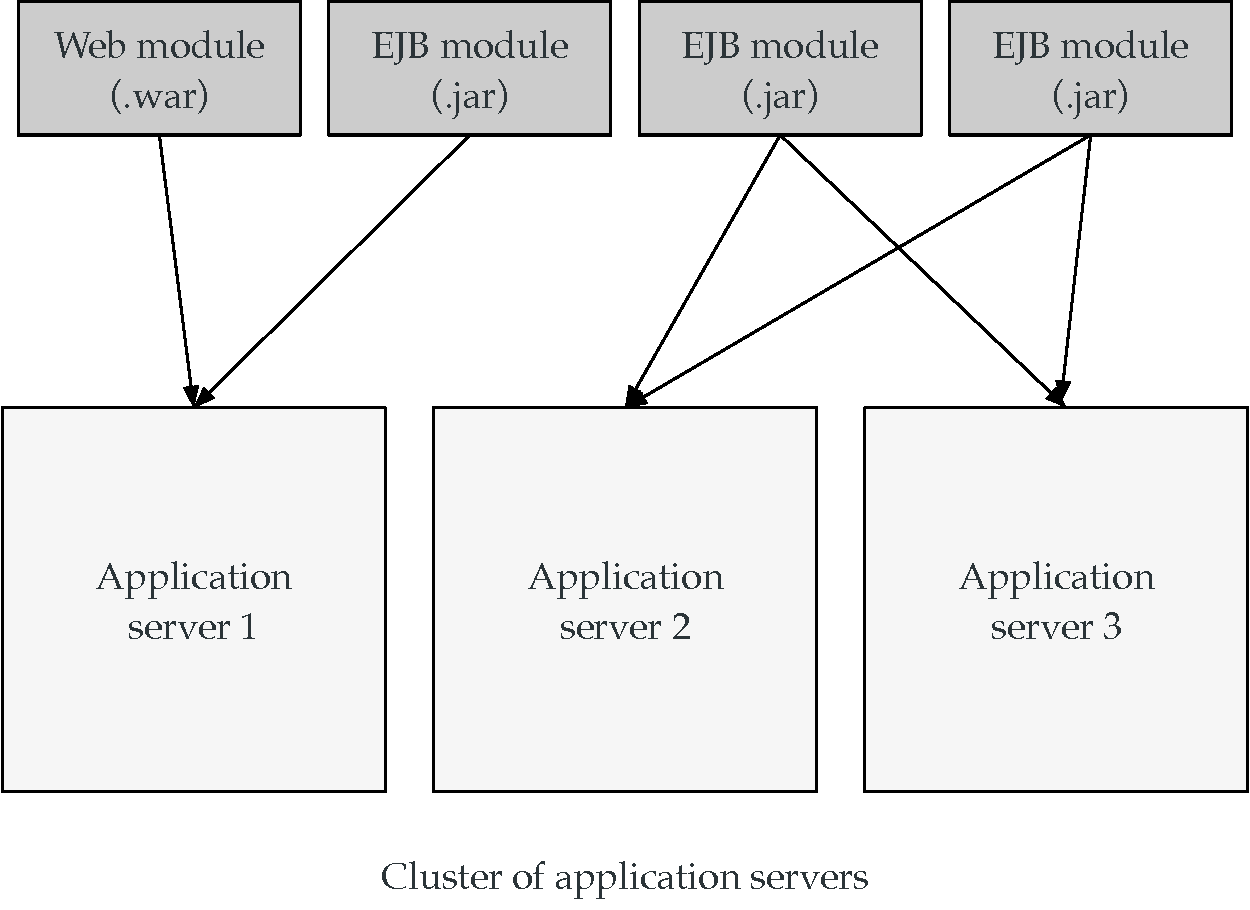
\includegraphics[width=0.8\linewidth]{Figures/deployment-ejb.pdf}
	\caption{Deployment of individual components in a cluster}
  \label{fig:deploymentEjb}
\end{figure}



\subsection{Types of Enterprise Java Beans}

\marginpar{Developers tend to use stateless session beans a lot more than stateful session beans. Message driven beans are very useful when the application has to be integrated with legacy applications. Entity beans have disappeared and been replaced with entities defined in the Java Persistence API.}

So far, we have used the term \ac{EJB} in a generic way, to refer to components that implement business services and that can be deployed in application servers. In fact, the specification defines several types of beans: \ac{SLSB}, \ac{SFSB}, \ac{MDB} and now defunct Entity Beans (not to be confused with entities in the \ac{JPA} specification.

\subsubsection{Stateless Session Beans}

These are the most commonly used \ac{EJB}s are used to implement services that do not maintain a conversational state. In other words, when every method call made by a client on a \ac{SLSB} is independent of the previous calls.

When creating a \ac{EJB}, one has to decide whether it will be accessed \emph{locally} (from servlets and other \ac{EJB}s in the same application), or \emph{remotely} (from rich clients and other applications). For many applications, the default choice is now to expose only a local interface. When the decision has been made, the interface can be created and annotated either with \texttt{@Local} and \texttt{@Remote}. The next step is to implement a Java class, which does not have to extend any class but has to be annotated with \texttt{@Stateless}. This is what will allow the application server to detect that the class is a managed component, which it must instantiate and control.

\marginpar{Since Java EE 6, it is not mandatory to explicitly local interfaces for \ac{SLSB}s and it is possible to only create a class. Still, we consider that it is a good practice to create interface files.}

\lstset{
	caption={Local interface defined for a stateless session bean},
	language=java,
	label={lst:localInterfaceSlsb}
}
\vspace{10pt}
\begin{minipage}{\linewidth}
\begin{lstlisting}[frame=single]
package ch.heigvd.amt.mvcsimple.business;

import javax.ejb.Local;

@Local
public interface ICustomerManager {

    public String generateCustomerId();

}
\end{lstlisting}
\end{minipage}

\lstset{
	caption={Stateless session bean implementation},
	language=java,
	label={lst:SlsbImplementation}
}
\vspace{10pt}
\begin{minipage}{\linewidth}
\begin{lstlisting}[frame=single]
package ch.heigvd.amt.mvcsimple.business;

import javax.ejb.Stateless;
import java.util.UUID;

@Stateless
public class CustomerManager implements ICustomerManager{

    @Override
    public String generateCustomerId() {
        return UUID.randomUUID().toString();
    }

}
\end{lstlisting}
\end{minipage}


\subsubsection{Stateful Session Beans}

\marginpar{Why manage conversational state in a SFSB rather than in an HTTP session? One argument is the need to support rich client that do not go through the presentation tier. Another argument is the separation of UI navigation state machines from business workflow state machines.}

\ac{SFSB}s are beans that manage conversational state. This means that some state is shared between the successive method call made by one client on the bean. For instance, it is possible to implement a shopping cart service, exposing methods like \texttt{void addProductToCart(Product p)} and \texttt{List<Product> getCartContent()}. Calling the first method 3 times before calling the second method shows that a state has to be managed during the conversation. Instead of storing it in the presentation tier or in the database, it is placed under the control of the \ac{SFSB}. This raises interesting questions in terms of resource consumption and scalability, which the specification addresses with mechanisms that we will not describe in details (e.g. \emph{passivation} and \emph{activation}).

\ac{SFSB}s are used much less often than \ac{SLSB}s. Even if there is often a need to manage conversational state, developers prefer to manage it in a different tier. They tend to either manage it in the presentation tier, with the HTTP session abstraction, or in the integration tier, with distributed data stores such as Redis. A couple of years ago, the JBoss Seam framework was perhaps the strongest advocate of \ac{SFSB}s and its documentation provides valuable information on the topic.


\subsubsection{Message Driven Beans}

\marginpar{MDBs are a great solution for integration with legacy applications and asynchronous task processing. In recent years, competing approaches have appeared in the NoSQL and big data space (redis, kafka, pulsar, etc.) }

\ac{MDB}s are very useful beans that are related to the \ac{JMS} specification, which deals with asynchronous messaging across components and applications. \ac{JMS} provides abstractions for point-to-point messaging (with queues) and publish-subscribe (with topics). A \ac{MDB} is a service that does not react to an incoming HTTP request or to a (remote) procedure call. It is a service that reacts to a message posted in a queue or broadcasted on a communication channel. It implements a single method, with the following signature: \texttt{public void onMessage(Message message)}. Messages exchanged via \ac{JMS} have a payload and metadata.

\begin{figure}[]
	\centering
    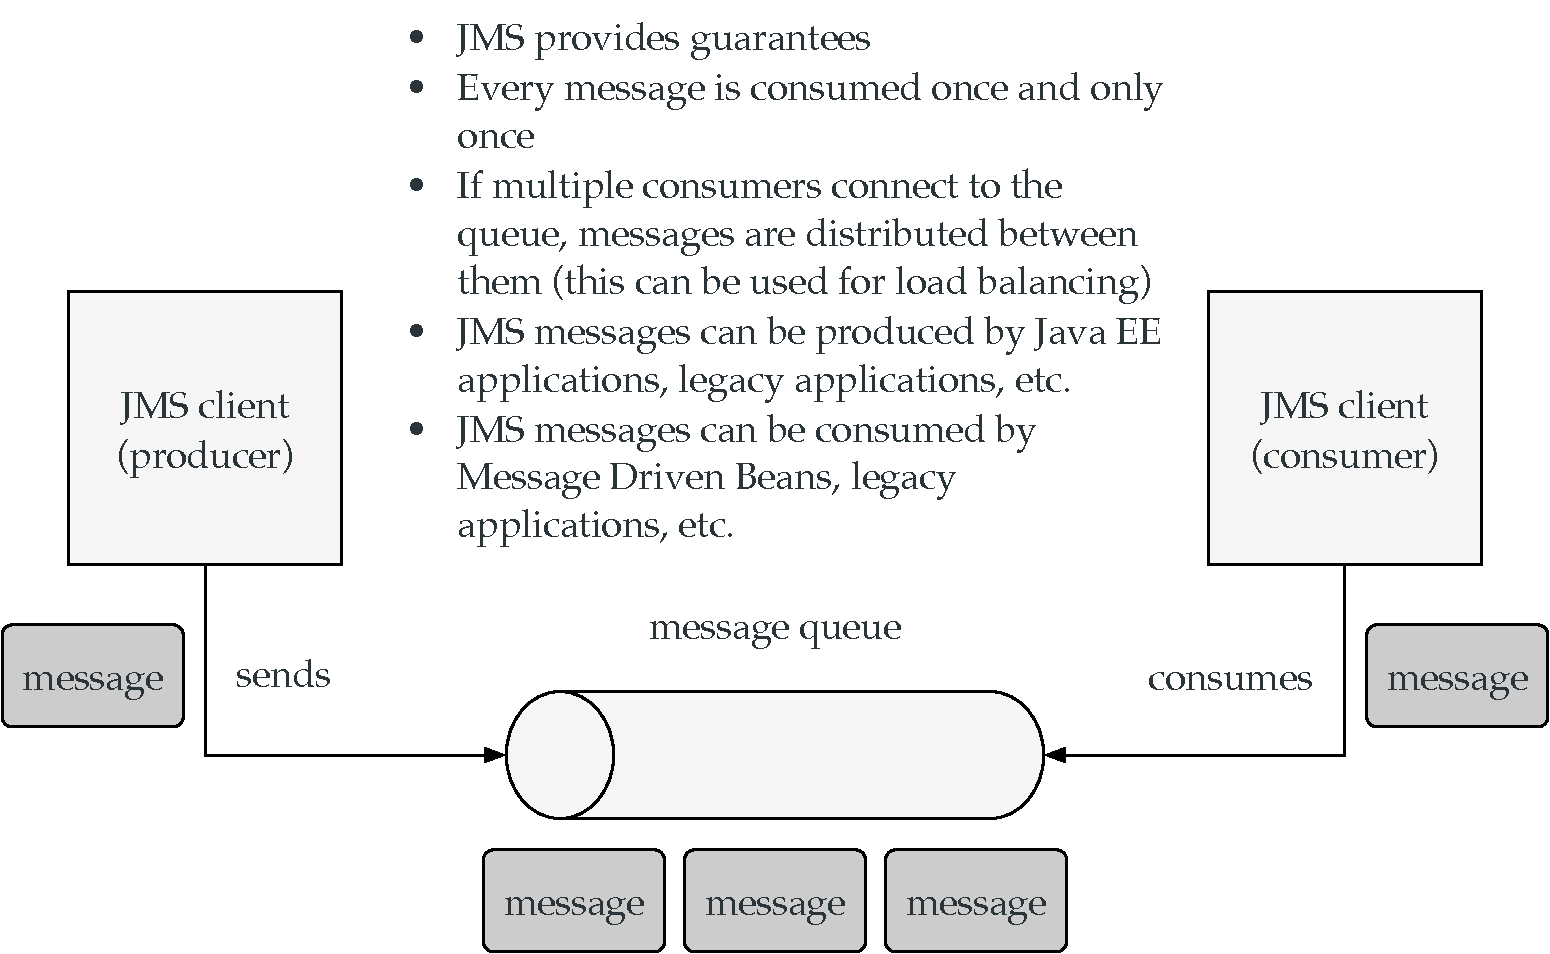
\includegraphics[width=1.0\linewidth]{Figures/jms-queue.pdf}
	\caption{Point-to-point communication with a JMS queue}
  \label{fig:jms-queue}
\end{figure}

\begin{figure}[]
	\centering
    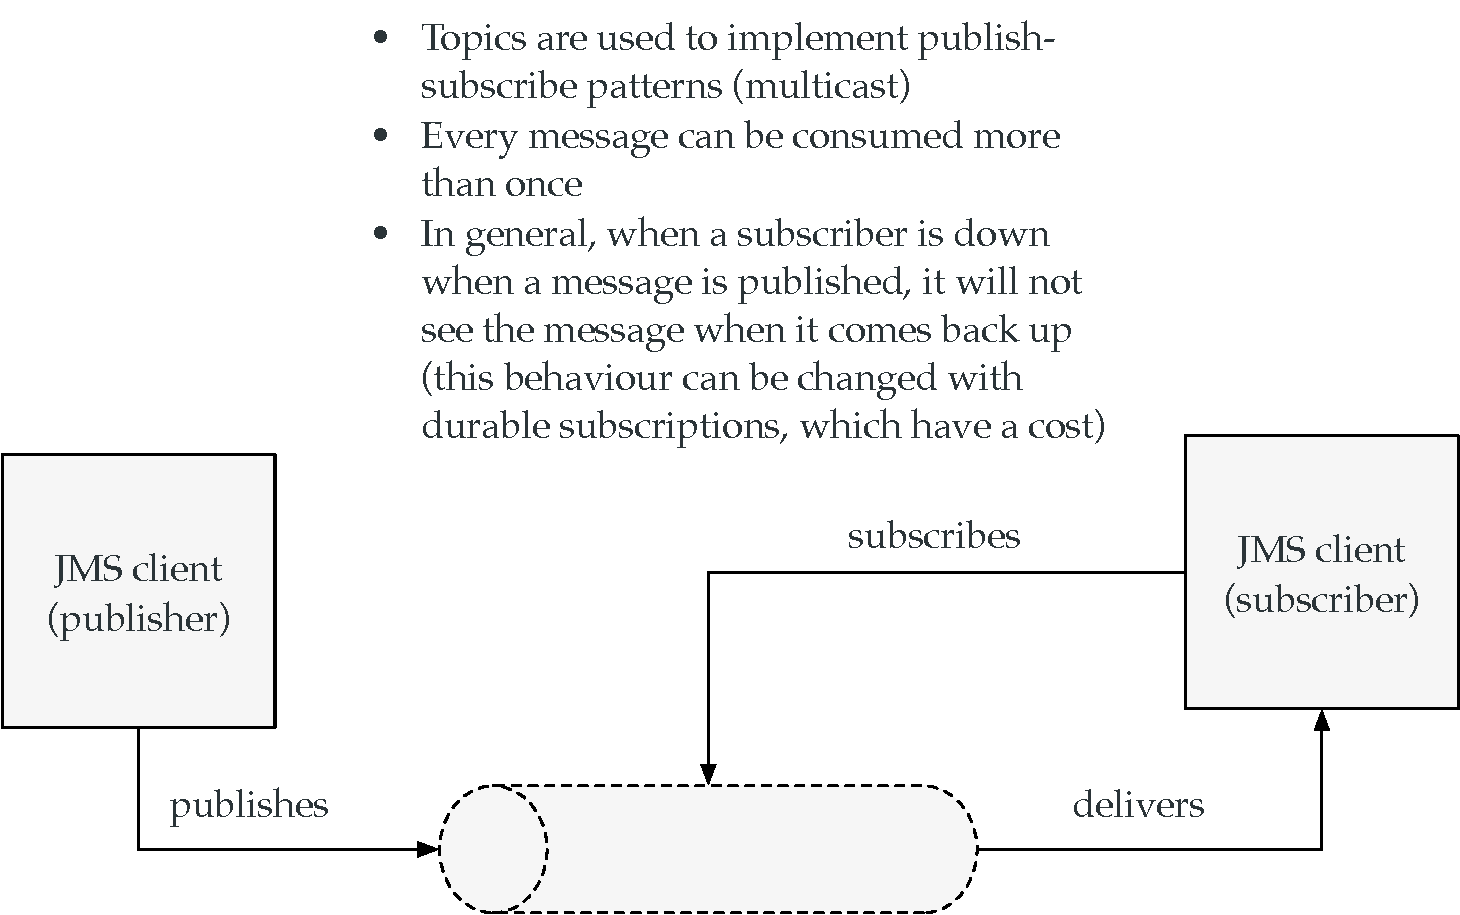
\includegraphics[width=1.0\linewidth]{Figures/jms-topic.pdf}
	\caption{Publish-Subscribe communication with a JMS topic}
  \label{fig:jms-topic}
\end{figure}

One common scenario to use \ac{MDB}s is the integration of a \ac{Java EE} application with other enterprise applications. For instance, think of a new application that needs to interact with a legacy application in a banking information system. Using a messaging system, with point-to-point queues or publish-subscribe channels is an approach with many benefits: low coupling, asynchronous interactions, etc.

Another common pattern is to implement a form of load balancing at the application level. Think of an application, where users can submit tasks (e.g. the task to look for a cheap flight, the task to generate a report, etc.). Instead of making a synchronous call to a service and to wait for an answer, it is often better to capture the task in an object and to process it asynchronously. A message queue can be used to notify worker nodes that tasks have been submitted. The semantics of JMS queues guarantee that every message posted to a queue will be consumed once and only once. If multiple workers connect to the same queue and consume messages, the system will deliver part of the messages to each worker. Hence, it is possible to scale an application by adding more worker nodes behind a queue. This is one reason for packaging and deploying \ac{MDB}s independently from a full enterprise archive (in other words, to package them in a separate \texttt{.jar} file and not within the \texttt{.ear} file).


\subsubsection{Entity Beans}

\marginpar{Entity beans were EJBs. They are not the same thing as entities defined in the Java Persistence API, which we will see later.}

Entity beans are a thing of the past. In the original specification, they were proposed as a way to interact with the database. They were a major pain to work with. This was true when designing the application, because they made it very hard to build an object-oriented domain model. This was also true when running the the application, because they raised a lot of performance issues.

The rapid success of the Hibernate \ac{ORM}, followed by the standard Java Persistence API, became the preferred way to interact with the database in Java EE. Entity beans can only be found in very old applications.

\section{Managed components}

To understand how \ac{EJB}s work and the value they add to \ac{POJO}s, it is first necessary to understand the concept of \emph{managed component}. This concept is related to the \ac{IoC} pattern that we have seen in the previous chapter. Remember that when we have introduced it, we have explained how application frameworks work and how they control the creation of classes and the invocation of methods provided by the developer.

\subsection{Lifecycle management}

\marginpar{The developer does not create instances of managed components: the framework does.}

Managed components have a well-defined \emph{lifecycle}, which can be described by a state machine. The \emph{state machine} specifies all the states in which the component can be, from its initial creation until its final destruction. The state machine also specifies what are the \emph{events} that cause state transitions and what is the origin of these events. We say that components are managed because the application developer is not responsible for controlling their lifecycle. The framework, in our case, the \ac{Java EE} container, is responsible for controlling it.

When we have studied the presentation tier, we have seen a first type of managed component: the servlets. Remember that in the code that we wrote, we implemented sub-classes of \texttt{HttpServlet}, but we never created instances of these classes. The application server took care of this task. The lifecycle of servlets is precisely described in the Servlet specification and this is how we can truly understand when servlet instances are created, how many instances are created and how they behave from a concurrency point of view. Understanding this lifecycle is mandatory to write correct and high-performance code. In the third part of the book, Section \ref{section:thread-safety-servlets-jmeter} describes an experiment that shows how misunderstandings can lead to bugs that manifest themselves under load.

\subsection{Resource pooling}

\marginpar{With a pool, it is possible to reuse objects that are expensive to create. It is also possible to limit the number of instances that can be created and to keep control of resources.}

Depending on the context, resource pooling can mean quite different things. Here, we are considering scenarios where special objects can be shared and reused across multiple invocations. Examples of objects that are often pooled include threads, database connections, network connections. There are different reasons why managing a pool of objects is interesting:

\begin{itemize}
\item It \emph{improves performance} when the creation of objects is expensive. A good example is a database connection. Creating one takes a lot of time, because it is necessary to establish a connection, to send credentials and to initialize the conversation. Instead of doing all that work for every client request, the idea is to keep several connections in a pool. When a new client request arrives, we can get a connection from the pool, use it to process the request and return it to the pool (without closing it).
\item It \emph{prevents resource exhaustion} and allows us to limit the rate at which client requests are served. In the example of database connections, if a new connection is opened for every client request, there is a risk to overload the database if many client requests arrive at the same time. A pool can be used to limit the concurrency: when a client request comes in and there is no connection available in the pool, then the request is placed in a queue until one becomes available.
\end{itemize}

The application server is managing \ac{EJB}s in pools. The behaviour of the EJB pools can be configured in the administration interface of the application server. Typically, the initial size of the pool, its maximum size, and what happens when the pool has been exhausted can be configured. This is an area where there are differences between application servers.

\subsection{Aspect oriented programming}

\marginpar{With AOP, it is possible to split the source code in multiple files. Functional aspects are implemented in one file, non-functional aspects are implemented in other files. This increases modularity, facilitates reuse and maintainability.}

One design goal for the \ac{Java EE} and the \ac{EJB} specifications was to facilitate \emph{separation of concerns}. Separation of concerns means that in a well-designed codebase, every unit should focus on a single task (a single concern, a single aspect). \ac{AOP} is a programming paradigm that supports this goal. \ac{EJB}s implement a basic form of \ac{AOP}. Other frameworks, such as AspectJ and the Spring framework, offer more advanced mechanisms.

Enterprise applications are complex for two reasons. Firstly, they are complex because they implement rich domain models, with a lot of business entities and processes. Secondly, they are complex because they have to fulfill non-functional requirements: security, availability, performance, etc. The skills needed to address these two types of complexity are very different. To address the first one, developers need deep business domain expertise. To address the second one, developers need deep technical expertise.

\begin{figure}[]
	\centering
    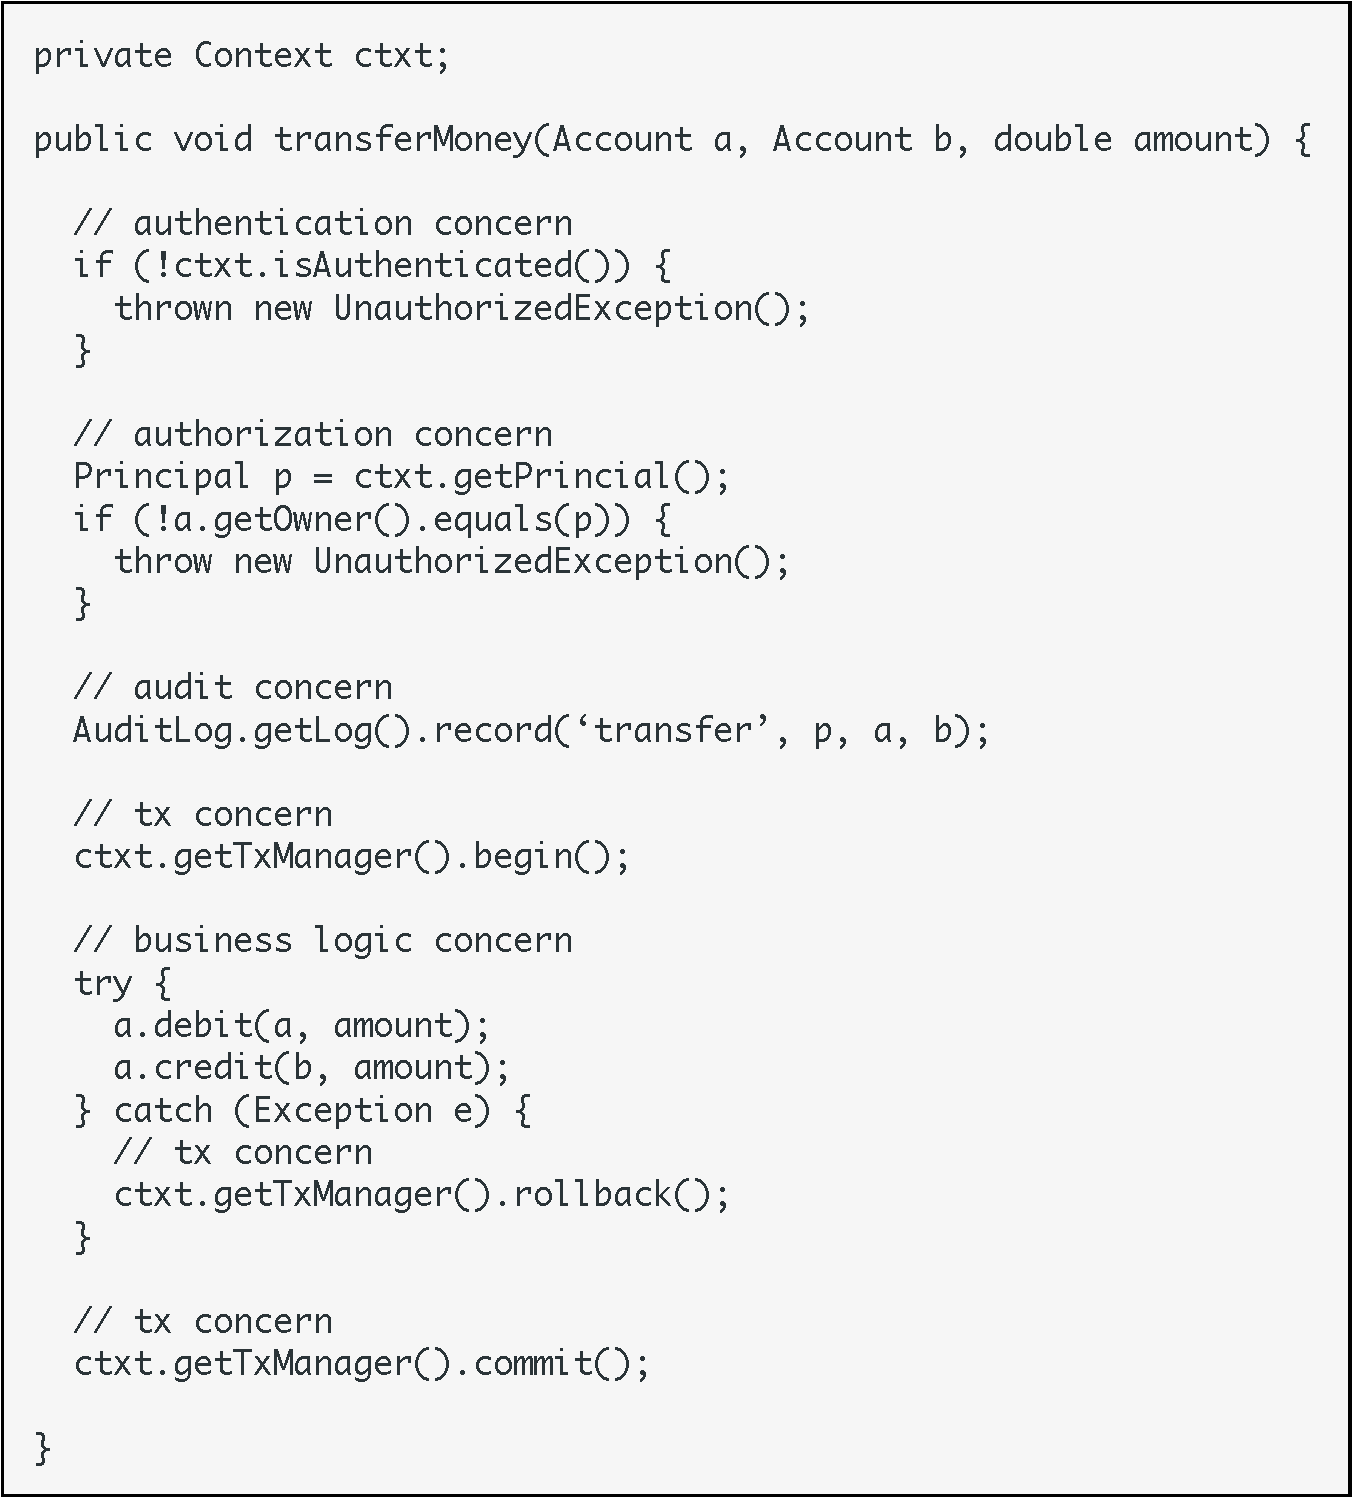
\includegraphics[width=0.8\linewidth]{Figures/aop-code-without.pdf}
	\caption{Code without separation of concerns}
  \label{fig:aop-without}
\end{figure}

\begin{figure}[]
	\centering
    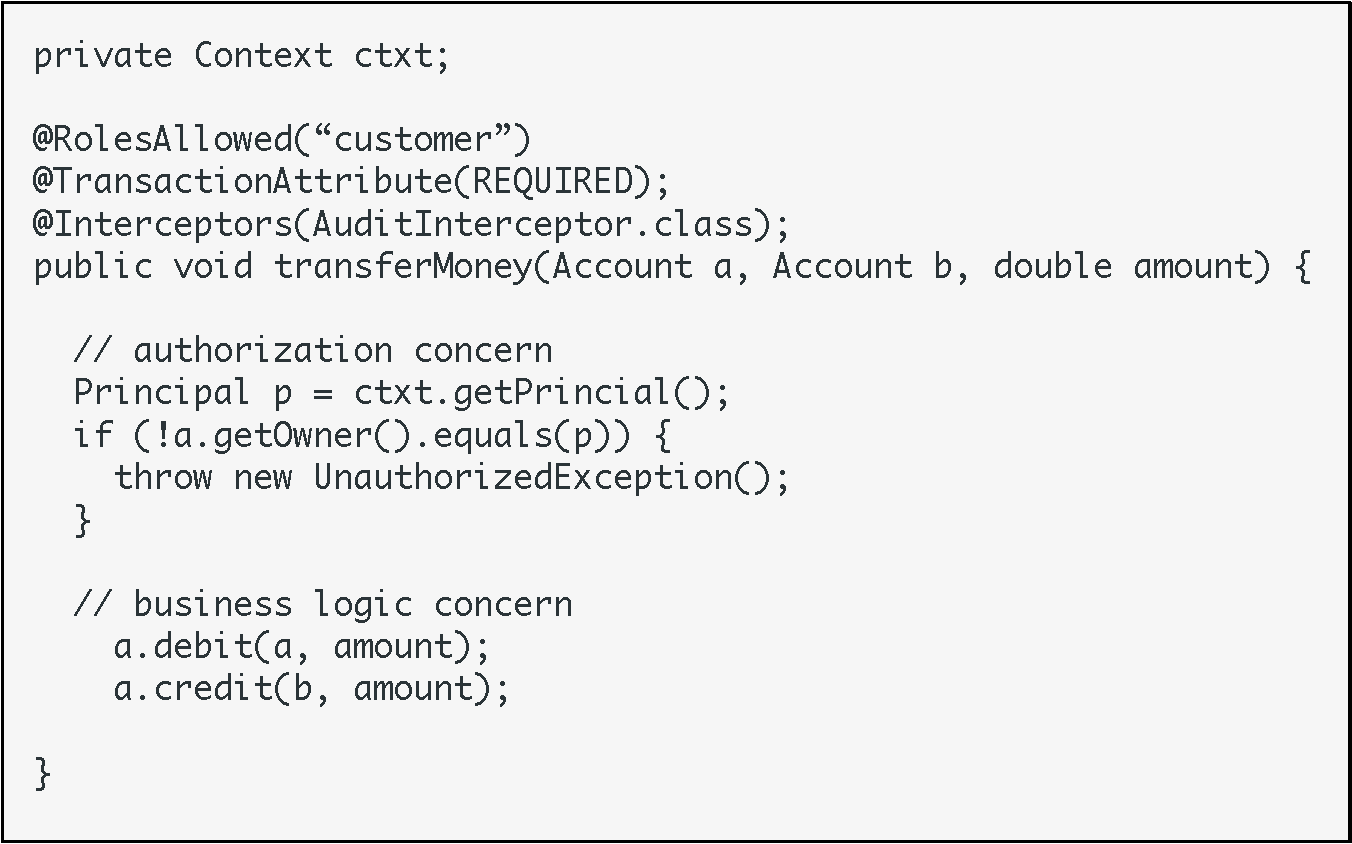
\includegraphics[width=0.8\linewidth]{Figures/aop-code-with.pdf}
	\caption{Code with separation of concerns}
  \label{fig:aop-with}
\end{figure}

Is there a way for a platform to take care of the technical complexity, thereby letting the developers focus only on the business complexity? This was the vision for the \ac{Java EE} platform: managed components were seen as a way to let the application server deal with the technical aspects, behind the scenes. The developers would merely have to \emph{declare their intents}, originally in deployment descriptors and later on in annotations. In reality, it is not possible to design a multi-tiered application without understanding distributed computing issues and tradeoffs. Application developers have to deal with \emph{some} of the technical complexity. But it is true that managed components, such as \ac{EJB}s, can \emph{reduce} the technical complexity and handle some of work.

To illustrate the notion of separation of concerns, let us compare the code in Figure \ref{fig:aop-without} and Figure \ref{fig:aop-with}. In the first case, we see that the business logic is lost in the middle of a lot of statements that deal with authentication, authorization, auditing and transaction management. The code is not easy to read and it is hard to grasp the business intent of the method at first glance. In the second case, the non-functional statements have been removed and replaced by annotations. In other words, the developer has used a way to declare how the method should behave from a security and transactional point of view. This is information that the developer gives to the application server, who will have the responsibility to enforce these policies. In the example, we see that some aspects can be declared with standard \ac{EJB} annotations (\texttt{@RolesAllowed} and \texttt{@TransactionAttribute}), while other aspects need to be handled by the developer but in a separate class: the \texttt{@Interceptor} annotation states that the class \texttt{AuditInterceptor}, provided by the developer, has to be applied as a filter when the method is invoked. This is an application of the pipes and filters pattern that we have seen in Section \ref{section:pipesAndFilters}.

\subsection{Aspect oriented programming: behind the scenes}

Using \ac{AOP} mechanisms when implementing \ac{EJB}s is fairly easy. One needs to know what aspects are supported by the platform and know which annotations are used to apply them. But it is also important to understand what happens behind the scenes. How is it possible for the container to apply these policies when a client invokes a method on an \ac{EJB}? 

The following experiment can reveal some of the work done by the application server. Run the application with the debugger enabled and simply put a breakpoint in the \ac{SLSB} method. Access the servlet that makes a call to the \ac{SLSB} and have a close look at the stack trace in your IDE. An example is shown in Figure \ref{fig:debugger-slsb}.

\marginpar{Never, ever, create an instance of an \ac{EJB} yourself. You would bypass the creation of a dynamic proxy and the magic would disappear.}

In this example, we see that two methods named \texttt{generateCustomerId()} have been called. As could be expected, one them is the method that we implemented in our \texttt{CustomerManager.java} class. The other, however, is not code that we wrote. Instead, we see that it is provided by a class named \texttt{\$Proxy344} in the \texttt{com.sun.proxy package}. The container uses the mechanism of \href{https://docs.oracle.com/javase/8/docs/technotes/guides/reflection/proxy.html}{dynamic proxies} offered by the Java platform. It can intercept every method call made to the bean and can inject additional logic.

\begin{figure}[]
	\centering
    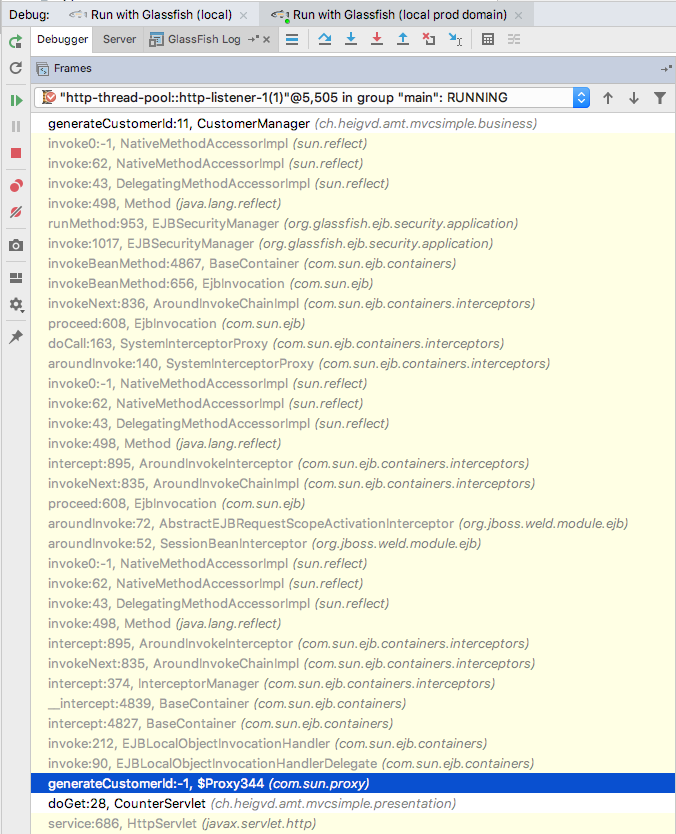
\includegraphics[width=0.9\linewidth]{Figures/debugger-slsb.png}
	\caption{The debugger reveals thE proxy created by the container}
  \label{fig:debugger-slsb}
\end{figure}

\section{The Dependency Injection pattern}

The last topic that we cover in this chapter is actually a generic design pattern, which can be applied in every tier of the architecture. For instance, on the client-side, the Javascript framework AngularJS makes extensive use of the pattern.

\marginpar{When object A calls a method on object B, we say that A depends on B. How does A obtain the reference to B?}

Before describing the pattern, it is necessary to clarify what we mean by \emph{dependency}. Our context is object-oriented programming. An object has a dependency on another object if at some point it needs to invoke one of this methods. For instance, a \texttt{CheckoutService} class might have a dependency on a \texttt{PriceCalculatorService} class: in an online shop, when you proceed to checkout, the price of your order needs to be computed (which can be a fairly sophisticated process with various policies and business rules). Very often, dependencies are not expressed on concrete classes, but rather on interfaces. In the previous example, this would make it possible to implement different pricing strategies in different classes and to select one of them at runtime.

Now that we know what a dependency is, we can explain what it means to \emph{inject} one.

\begin{itemize}
\item An example of code that does not use dependency injection is shown in Listing \ref{lst:dependencyInstantiation}. In this case, the \texttt{CheckoutService} obtains its dependency by instantiating it itself. This creates a tight coupling between the two classes and does not make it possible to switch the implementation at runtime.
\item A better approach is shown in Listing \ref{lst:dependencyLookup}. In this case, the client uses a service registry and performs a lookup operation. It asks the registry to obtain a reference to the dependency by providing a service name. This technique was the standard way to manage dependencies between servlets and \ac{EJB}s in the first versions of the platform.
\item Finally, dependency injection is shown in List \ref{lst:dependencyInjection}. In this case, the developer only declares that the checkout service has a dependency on the pricing service. He uses an annotation provided by the dependency injection framework (for a \ac{Java EE} container, he uses the \texttt{@EJB} annotation). This works if and only if the services are managed components, whose lifecycle is controlled by the container. At runtime, the container creates instances of \texttt{CheckoutService} and of an implementation of\texttt{IPricingService}. It scans the annotations and sees that it must inject a reference to the second instance in the first instance. How this is done depends on the technology and framework, but common techniques are \emph{constructor-based dependency injection} (the constructor of the dependent class includes a parameter so that a reference to the dependency can be passed) and \emph{setter-based dependency injection} (a setter method is provided by the developer and invoked by the framework).
\end{itemize}

\marginpar{Once again: never, ever, create an instance of an \ac{EJB} yourself. Either use dependency injection or do a lookup in the naming registry.}

Last but not least, Listing \ref{lst:dependencyInjectionServletEJB} shows a concrete application of dependency injection in the \ac{Java EE} platform. The container is managing two components: a servlet and a \ac{SLSB}. The developer has expressed the fact that the servlet depends on the \ac{SLSB} by using the \texttt{@EJB} annotation in the servlet. This is what allows the container to figure out what needs to be done and how it should wire the components together.

\lstset{
	caption={Bad practice: dependency is instantiated by the client service},
	language=java,
	label={lst:dependencyInstantiation}
}
\vspace{10pt}
\begin{minipage}{\linewidth}
\begin{lstlisting}[frame=single]
package ch.heigvd.amt.mvcsimple.business;

public class CheckoutService {

    private IPricingService pricingService;

    public CheckoutService() {
        pricingService = new PricingServiceImpl1();
    }

    public void checkout(Cart cart) {
        pricingService.computePrice();
    }

}
\end{lstlisting}
\end{minipage}


\lstset{
	caption={Better practice: dependency is looked up in a registry},
	language=java,
	label={lst:dependencyLookup}
}
\vspace{10pt}
\begin{minipage}{\linewidth}
\begin{lstlisting}[frame=single]
package ch.heigvd.amt.mvcsimple.business;

public class CheckoutService {

    private IPricingService pricingService;

    public CheckoutService() {
        pricingService = (IPricingService) ServiceRegistry.lookup("pricing-service-policy-xy");
    }

    public void checkout(Cart cart) {
        pricingService.computePrice();
    }

}
\end{lstlisting}
\end{minipage}

\lstset{
	caption={Dependency is injected by the framework as part of the lifecycle},
	language=java,
	label={lst:dependencyInjection}
}
\vspace{10pt}
\begin{minipage}{\linewidth}
\begin{lstlisting}[frame=single]
package ch.heigvd.amt.mvcsimple.business;

public class CheckoutService {

    @AnnotationProvidedByTheDependencyInjectionFramework
    private IPricingService pricingService;

    public CheckoutService() {
    }

    public void checkout(Cart cart) {
        pricingService.computePrice();
    }

}\end{lstlisting}
\end{minipage}


\lstset{
	caption={Injecting a reference to a SLSB into a servlet},
	language=java,
	label={lst:dependencyInjectionServletEJB}
}
\vspace{10pt}
\begin{minipage}{\linewidth}
\begin{lstlisting}[frame=single]
package ch.heigvd.amt.mvcsimple.presentation;

import ch.heigvd.amt.mvcsimple.business.ICustomerManager;

import javax.ejb.EJB;
import javax.servlet.ServletException;
import javax.servlet.annotation.WebServlet;
import javax.servlet.http.HttpServlet;
import javax.servlet.http.HttpServletRequest;
import javax.servlet.http.HttpServletResponse;
import java.io.IOException;

@WebServlet(name = "UserManagerServlet", urlPatterns = "/users")
public class UserManagerServlet extends HttpServlet {
    
    @EJB
    ICustomerManager customerManager;

    protected void doGet(HttpServletRequest request, HttpServletResponse response) throws ServletException, IOException {
        String newCustomerId = customerManager.generateCustomerId();
        request.setAttribute("newCustomerId", newCustomerId);
        request.getRequestDispatcher("/some/view").forward(request, response);

    }
}\end{lstlisting}
\end{minipage}



\section{Questions}

To answer these questions, you will need to have read the chapter but also to have done some research. Make sure that you are able to answer every question. Discuss your responses with your peers.


